\section*{Appendix}
\label{sec:appendix}

\addcontentsline{toc}{part}{Appendix}

\startcontents[appendix]
\begingroup
\hypersetup{linkcolor=promptblue}
\printcontents[appendix]{}{1}{\section*{Appendix Contents}}
\endgroup




\section{Preliminary of Reinforcement Learning}
\label{apdx:rl}

This section details the reinforcement learning (RL) preliminaries underpinning our multi-turn training objective. We first review the standard Group Relative Policy Optimization (GRPO) algorithm~\citep{shao2024deepseekmath}, which operates on single-turn generations. Subsequently, we describe its extension to search-augmented rollouts, as introduced by Search-R1~\citep{jin2025searchr1trainingllmsreason}, wherein the policy interleaves generation with calls to an external search engine. These formulations serve as the direct precursors to the multi-turn, multi-tool objective employed by \textsc{OpenSearch-VL} (see Sec.~\ref{sec:multi-turn-grpo}).

\subsection{Standard GRPO}

GRPO~\citep{shao2024deepseekmath} is an actor-critic variant of Proximal Policy Optimization (PPO)~\citep{schulman2017proximal} that eliminates the reliance on a learned value function. Instead of maintaining a separate critic model to estimate a baseline, GRPO derives its advantage estimate by comparing multiple responses sampled for the same prompt, collectively defining a \emph{group}. This parameter-efficient design is particularly advantageous in settings where only a scalar outcome-level reward is available, reducing memory overhead and mitigating the instability of training a dense token-level value function.

Formally, given a prompt distribution $\mathcal{D}$ and a reference policy $\pi_{\theta_{\text{old}}}$, GRPO samples a group of $G$ candidate responses $\{o_1, o_2, \dots, o_G\} \sim \pi_{\theta_{\text{old}}}(\cdot \mid q)$ for each prompt $q \sim \mathcal{D}$. Each response is evaluated via a reward function $r_i = r(q, o_i)$. To compute the advantages, GRPO standardizes these rewards within the local group:
\begin{equation}
    \hat{A}_{i,t} \;=\; \widetilde{r}_i \;=\; \frac{r_i - \mathrm{mean}(\{r_j\}_{j=1}^G)}{\mathrm{std}(\{r_j\}_{j=1}^G)},
    \quad \text{for all tokens } t = 1, \dots, |o_i|.
    \label{eq:grpo-advantage}
\end{equation}
By this formulation, all constituent tokens of a given response $o_i$ are assigned a uniform advantage scalar. The policy parameters $\theta$ are subsequently optimized by maximizing the clipped surrogate objective:
\begin{equation}
\begin{aligned}
    \mathcal{J}_{\text{GRPO}}(\theta)
    \;=\;&\;\; \mathbb{E}_{q \sim \mathcal{D},\, \{o_i\}_{i=1}^G \sim \pi_{\theta_{\text{old}}}(\cdot \mid q)} \Bigg[
    \frac{1}{G} \sum_{i=1}^{G} \frac{1}{|o_i|} \sum_{t=1}^{|o_i|} \bigg\{ \\
    &\quad\; \min\!\Big( \rho_{i,t}(\theta)\,\hat{A}_{i,t},\;\;
    \mathrm{clip}\bigl(\rho_{i,t}(\theta),\,1{-}\epsilon,\,1{+}\epsilon\bigr)\,\hat{A}_{i,t} \Big) \\
    &\quad\; -\; \beta\, \mathbb{D}_{\text{KL}}\!\bigl[\pi_\theta \,\|\, \pi_{\text{ref}}\bigr] \bigg\} \Bigg],
\end{aligned}
\label{eq:grpo-objective}
\end{equation}
where the importance sampling ratio is defined as
\begin{equation}
    \rho_{i,t}(\theta) \;=\; \frac{\pi_\theta(o_{i,t} \mid q,\, o_{i,<t})}{\pi_{\theta_{\text{old}}}(o_{i,t} \mid q,\, o_{i,<t})}.
\end{equation}
Here, $\epsilon$ represents the probability ratio clipping hyperparameter, and $\beta$ modulates the Kullback--Leibler (KL) divergence penalty against a fixed reference policy $\pi_{\text{ref}}$. In contrast to standard PPO---which subsumes the KL penalty directly into the reward signal and necessitates a parameterized value network to approximate $\hat{A}_{i,t}$~\citep{schulman2017proximal}---GRPO enforces the KL regularization explicitly within the loss landscape. By deriving $\hat{A}_{i,t}$ strictly from empirical group statistics (Eq.~\ref{eq:grpo-advantage}), GRPO naturally aligns with the comparative structure of preference-based reward modeling.

\subsection{GRPO with Search Engine}

Search-R1~\citep{jin2025searchr1trainingllmsreason} extends the GRPO framework from unimodal, single-turn generation to an interleaved, search-augmented generative process. Rather than sampling an isolated response $o_i \sim \pi_{\theta_{\text{old}}}(\cdot \mid q)$, Search-R1 generates a multi-step rollout comprising both policy-emitted tokens and external evidence retrieved from a search engine $\mathcal{R}$. This search-augmented sampling distribution is denoted as:
\begin{equation}
    o_i \;\sim\; \pi_{\theta_{\text{old}}}(\cdot \mid q; \mathcal{R}) \;=\; \pi_{\theta_{\text{old}}}(\cdot \mid q) \,\bigotimes\, \mathcal{R},
\end{equation}
where $\bigotimes$ represents the interleaving operator: whenever the policy emits a search command, the retrieved documents are appended to the conditioning context, and the policy resumes generation conditioned on this expanded prefix.

To prevent the optimizer from erroneously updating parameters based on exogenous environmental tokens, Search-R1 utilizes a masking function that filters out non-generated tokens. Defining $M_{\text{gen}}(y_{i,t}) \in \{0, 1\}$ as an indicator variable where $M_{\text{gen}}(y_{i,t}) = 1$ if $y_{i,t}$ is explicitly generated by the policy, the corresponding Search-R1 GRPO objective becomes:
\begin{equation}
\begin{aligned}
    \mathcal{J}_{\text{GRPO}}^{\mathcal{R}}(\theta)
    \;=\;&\;\; \mathbb{E}_{q \sim \mathcal{D},\, \{o_i\}_{i=1}^{G} \sim \pi_{\theta_{\text{old}}}(\cdot\mid q;\,\mathcal{R})}
    \Bigg[
    \frac{1}{G} \sum_{i=1}^{G}
    \frac{1}{\sum_{t=1}^{|o_i|} M_{\text{gen}}(y_{i,t})}
    \sum_{\substack{t=1 \\ M_{\text{gen}}(y_{i,t})=1}}^{|o_i|} \bigg\{ \\
    &\quad\; \min\!\Big( \rho_{i,t}^{\mathcal{R}}(\theta)\,\hat{A}_{i,t},\;\;
    \mathrm{clip}\bigl(\rho_{i,t}^{\mathcal{R}}(\theta),\,1{-}\epsilon,\,1{+}\epsilon\bigr)\,\hat{A}_{i,t} \Big) \\
    &\quad\; -\; \beta\, \mathbb{D}_{\text{KL}}\!\bigl[\pi_\theta \,\|\, \pi_{\text{ref}}\bigr] \bigg\} \Bigg],
\end{aligned}
\label{eq:grpo-search}
\end{equation}
featuring the environment-conditioned importance ratio:
\begin{equation}
    \rho_{i,t}^{\mathcal{R}}(\theta) \;=\; \frac{\pi_\theta(y_{i,t} \mid q,\, y_{i,<t};\, \mathcal{R})}{\pi_{\theta_{\text{old}}}(y_{i,t} \mid q,\, y_{i,<t};\, \mathcal{R})}.
\end{equation}
Relative to standard GRPO (Eq.~\ref{eq:grpo-objective}), this adaptation introduces two pivotal modifications. First, the expectation is calculated with respect to the interleaved distribution $\pi_{\theta_{\text{old}}}(\cdot \mid q; \mathcal{R})$, ensuring the causal conditioning history incorporates all previously retrieved external evidence. Second, the objective is normalized strictly by the count of generated tokens, $\sum_t M_{\text{gen}}(y_{i,t})$, restricting gradient calculations to policy-authored positions. Equivalently masking the KL divergence ensures the model is not penalized for distributional divergence over environmental observations. These mechanisms adapt GRPO to tool-in-the-loop architectures and establish the theoretical foundation for our multimodal environment $\mathcal{E}$ formulation (Sec.~\ref{sec:multi-turn-grpo}).

\section{Multi-Turn Search Fatal-Aware GRPO Details}
\label{apdx:grpo-detail}



Building upon the foundations established in Appendix~\ref{apdx:rl}, this section details the mechanics of our multi-turn, search-augmented RL objective introduced in Sec.~\ref{sec:multi-turn-grpo}. We articulate the detection logic for fatal execution cascades and rigorously derive the advantage estimation process incorporating one-sided clamping; the composite reward $r(\tau)$ and its three components $r_{\text{fmt}},\, r_{\text{acc}},\, r_{\text{query}}$ are defined directly in Sec.~\ref{sec:multi-turn-grpo}.

\begin{figure}[t]
  
  \centering
  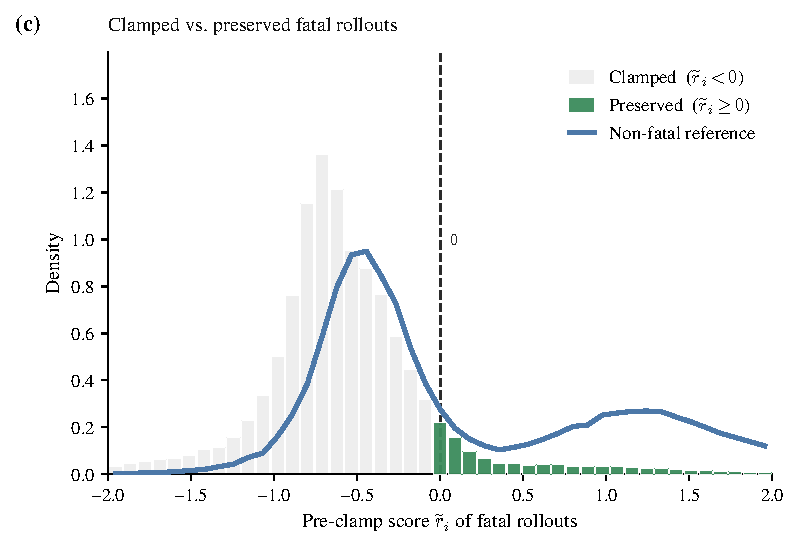
\includegraphics[width=0.6\linewidth]{figures/fatal_clamping_aggregate.pdf}
  \caption{%
    \textbf{Aggregate distribution of clamped and preserved fatal rollouts.}
    Pre-clamp group-normalized scores $\widetilde{r}_i$ aggregated over
    $10{,}000$ groups ($G{=}16$; $47{,}978$ fatal rollouts in total).
    $91.8\%$ of fatal rollouts fall on the negative side of the clamp
    threshold (mean $\overline{\widetilde{r}}_{-}{=}-0.68$) and are zeroed
    out by $\hat{A}_i{=}\max(\widetilde{r}_i,0)$; the remaining $8.2\%$ are
    preserved (mean $\overline{\widetilde{r}}_{+}{=}+0.57$) and overlap with
    the positive mode of the non-fatal reference density (blue line:
    pre-clamp scores of all non-fatal rollouts from the same groups).
    Preservation is therefore driven by the same group-normalized score that
    GRPO already computes, and the preserved fatal prefixes sit in the same
    score regime as stronger non-fatal behaviors -- not an ad-hoc heuristic.%
  }
  \label{fig:fatal-clamping-aggregate}
  
\end{figure}

\subsection{Fatal Step Detection Logic}
\label{apdx:fatal-detail}

Unconstrained interactions with external environments inevitably yield ``fatal'' states---irrecoverable error cascades rendering subsequent reasoning invalid. We articulate the procedure for computing the fatal step index $f_i$, which drives the fatal-aware token mask (Eq.~\ref{eq:fatal-mask}).

For a given trajectory $\tau_i$ of length $L_i$, we instantiate a stateful error counter $n_{\text{err}}$ initialized to zero. At each sequential step $l \in \{0, 1, \dots, L_i\}$, the counter transitions according to:
\begin{equation}
  n_{\text{err}}^{(l)} \;=\;
  \begin{cases}
    n_{\text{err}}^{(l-1)} + 1 & \text{if step } l \text{ triggers a tool-execution error},\\
    0 & \text{otherwise}.
  \end{cases}
\end{equation}
The fatal step index is subsequently defined as the earliest step where the error threshold is breached:
\begin{equation}
    f_i = \min\{l : n_{\text{err}}^{(l)} = K\}.
\end{equation}
In our implementation, we set $K=3$. If the threshold is never reached, the trajectory is classified as non-fatal, denoted by setting $f_i = L_i+1$. 

This formulation embodies two critical design properties. First, the explicit reset condition ($n_{\text{err}}^{(l)} = 0$) ensures that \emph{isolated} transient errors---which are ubiquitous and often recoverable in realistic web environments---do not prematurely abort the trajectory. Second, the conservative threshold ($K=3$) dictates that a trajectory is only deemed fatal following three \emph{consecutive} failures, affording the autoregressive policy a robust opportunity to self-correct prior to gradient masking. Tool-execution errors triggering this counter encompass timeouts, malformed API payloads, and argument-parsing failures; these are flagged deterministically by the execution sandbox, independent of any learned heuristic.

\subsection{Advantage Derivation with One-Sided Clamping}
\label{apdx:advantage-detail}

We rigorously detail the advantage estimation protocol underpinning the objective function in Eq.~\ref{eq:our-grpo}.

\paragraph{Step 1: Unbiased Group Statistics.}
For a sampled group of $G$ rollouts originating from the identical prompt $(I_0, q)$, the empirical group mean and standard deviation are computed over the composite rewards:
\begin{equation}
  \mu_{\mathcal{G}} \;=\; \operatorname{sg}\!\left( \frac{1}{G}\sum_{j=1}^{G} r(\tau_j) \right), \qquad
  \sigma_{\mathcal{G}} \;=\; \operatorname{sg}\!\left( \sqrt{ \frac{1}{G}\sum_{j=1}^{G} \bigl(r(\tau_j) - \mu_{\mathcal{G}}\bigr)^{2} } \right).
\end{equation}
Here, $\operatorname{sg}(\cdot)$ denotes the stop-gradient operator. Consequently, $\mu_{\mathcal{G}}$ and $\sigma_{\mathcal{G}}$ act as static normalizing constants during backpropagation. Gradients flow exclusively through the importance sampling ratios evaluated on the unmasked, policy-generated tokens.

\paragraph{Step 2: Universal Group Normalization.}
Each trajectory within the group is assigned a standardized reward:
\begin{equation}
  \widetilde{r}_i \;=\; \frac{r(\tau_i) - \mu_{\mathcal{G}}}{\sigma_{\mathcal{G}} + \delta},
\end{equation}
where $\delta > 0$ provides numerical stability. Crucially, all $G$ trajectories---expressly including those truncated by the fatal condition ($f_i \le L_i$)---are incorporated into the calculation of $\mu_{\mathcal{G}}$ and $\sigma_{\mathcal{G}}$. This deliberate inclusion ensures that fatal trajectories actively shape the group-level baseline, anchoring the relative performance ranking across the entire sampled cohort.

\paragraph{Step 3: Fatal-Aware One-Sided Clamping.}
The standardized rewards are mapped to the final advantage estimates $\hat{A}_i$ via a piecewise clamping function:
\begin{equation}
  \hat{A}_i \;=\;
  \begin{cases}
    \widetilde{r}_i & \text{if } f_i = L_i{+}1 \quad\text{(non-fatal trajectory)},\\[4pt]
    \max\!\bigl(\widetilde{r}_i,\; 0\bigr) & \text{if } f_i \le L_i \quad\text{(fatal trajectory)}.
  \end{cases}
\end{equation}


\paragraph{Step 4: Gradient Dominance over Hard-Masking.}
We now formalize the informal claim that fatal-aware clamping strictly dominates the hard-masking baseline of~\citep{huang2026vision} in gradient informativeness. Let
\begin{equation}
  g_i^{\text{ours}} \;=\; \frac{1}{\sum_{t} M_{i,t}} \sum_{t=1}^{|\tau_i|} M_{i,t}\, \nabla_\theta \log \pi_\theta\!\bigl(y_{i,t} \mid h_{s(t)}\bigr)\, \hat{A}_i
  \label{eq:per-traj-grad}
\end{equation}
denote the (un-clipped) per-trajectory contribution to $\nabla_\theta \mathcal{J}(\theta)$ under our scheme, and let $g_i^{\text{hard}}$ denote the corresponding contribution under the hard-masking baseline, which discards every fatal trajectory in full so that $g_i^{\text{hard}} = 0$ whenever $f_i \le L_i$. We compare the two on the support of fatal trajectories.

\begin{proposition}[Dominance over hard-masking]
\label{prop:dominance}
Fix any fatal trajectory $\tau_i$ ($f_i \le L_i$). Then:
\begin{enumerate}[leftmargin=*,itemsep=1pt,topsep=1pt]
  \item If $\widetilde{r}_i < 0$, then $g_i^{\text{ours}} = g_i^{\text{hard}} = 0$.
  \item If $\widetilde{r}_i \ge 0$, then $g_i^{\text{hard}} = 0$, while $g_i^{\text{ours}}$ coincides with the search-augmented GRPO gradient (Eq.~\ref{eq:grpo-search}) of $\tau_i$ restricted to its viable prefix $\{t : s(t) < f_i,\; M_{\text{gen}}(y_{i,t}) = 1\}$, evaluated at the non-negative advantage $\widetilde{r}_i$.
\end{enumerate}
Consequently, $g_i^{\text{ours}}$ is weakly informative-dominant over $g_i^{\text{hard}}$: it never propagates gradient through the post-fatal suffix, never penalises the viable prefix, and strictly extracts positive reinforcement on prefixes whose group-normalised return exceeds the baseline.
\end{proposition}

\begin{proof}
By Eq.~\ref{eq:advantage}, $\widetilde{r}_i < 0$ implies $\hat{A}_i = 0$, so the surrogate term and its gradient vanish identically in Eq.~\ref{eq:per-traj-grad}; combined with $g_i^{\text{hard}} = 0$ by definition of hard-masking, this establishes (i). For $\widetilde{r}_i \ge 0$, $\hat{A}_i = \widetilde{r}_i$, while the fatal-aware mask $M_{i,t} = M_{\text{gen}}(y_{i,t}) \cdot \mathbb{1}[s(t) < f_i]$ retains exactly the policy-generated tokens of the viable prefix and zeros out (a) environment-emitted tokens and (b) all post-fatal tokens. On this support the per-token integrand of Eq.~\ref{eq:per-traj-grad} reduces token-by-token to that of Eq.~\ref{eq:grpo-search} with the same importance ratio $\rho_{i,t}$ and advantage $\widetilde{r}_i \ge 0$, so the per-token surrogates---and hence their gradients---agree. Since $g_i^{\text{hard}} = 0$ by definition, this establishes (ii).
\end{proof}

In aggregate, the one-sided clamp safely ignores invalid credit assignment while selectively harvesting positive reinforcement from prematurely truncated yet high-quality exploratory rollouts.

\paragraph{Bias of Group Statistics under Clamping.}
The asymmetric definition of $\hat{A}_i$ deserves an honest accounting. We compute $(\mu_\mathcal{G},\sigma_\mathcal{G})$ in Step~1 over \emph{all} $G$ rollouts---including fatal ones---so the standardised score $\widetilde{r}_i$ is zero-mean within the group; Step~3 then maps any negative $\widetilde{r}_i$ on a fatal trajectory to zero. Letting $\mathcal{F} \subseteq \{1,\dots,G\}$ index the fatal subset of the group,
\begin{equation}
  \frac{1}{G}\sum_{i=1}^{G} \hat{A}_i \;=\; \underbrace{\frac{1}{G}\sum_{i=1}^{G} \widetilde{r}_i}_{=\,0} \;+\; \underbrace{\frac{1}{G}\sum_{i \in \mathcal{F}} \max\!\bigl(0,\,-\widetilde{r}_i\bigr)}_{\;=\,b_\mathcal{G}\,\ge\,0},
  \label{eq:clamp-bias}
\end{equation}
so the clamp induces a non-negative bias $b_\mathcal{G}$ relative to the zero-mean GRPO baseline, in exchange for non-zero gradient on viable prefixes. We argue this trade-off is benign in our regime for two reasons. (a)~\emph{Concentration of fatal rollouts in the lower mode.} Figure~\ref{fig:fatal-clamping-aggregate} shows that $91.8\%$ of fatal rollouts have $\widetilde{r}_i < 0$ and are clamped to zero, while the residual $8.2\%$ that survive sit in the same score regime as competitive non-fatal rollouts; $b_\mathcal{G}$ is therefore dominated by samples whose viable prefix is empirically high-quality, rather than by indiscriminate inflation of low-quality fatals. (b)~\emph{Preservation of relative ranking.} Because $b_\mathcal{G}$ shifts only the fatal subset upward and never displaces non-fatal advantages, the within-group ordering between non-fatal trajectories---which is the actual signal GRPO exploits---remains intact. We therefore interpret $b_\mathcal{G}$ as a controlled positive bias that buys back gradient on prematurely truncated yet promising prefixes; replacing the clamp with an unbiased estimator (e.g., a separate baseline computed only over non-fatal rollouts, or a doubly-robust correction for $b_\mathcal{G}$) is an interesting alternative we leave for future work.

A sanity check of the resulting clamping behaviour, including a per-group-difficulty breakdown and the aggregate score distribution over $10{,}000$ groups, is reported in Sec.~\ref{sec:experiments} (Figs.~\ref{fig:fatal-clamping-cases} and~\ref{fig:fatal-clamping-aggregate}).




\section{Implementation Details}
\label{apdx:implementation-details}

Our agentic SFT pipeline builds on \textsc{LlamaFactory}~\citep{zheng2024llamafactory}, which we extend with multi-turn, tool-interleaved data collators and a Qwen3-VL-aware vision/text packing scheme so that interleaved image observations produced by visual tools (\textsc{Crop}, \textsc{Sharpen}, \textsc{SuperResolution}, \textsc{PerspectiveCorrect}, \textsc{OCR}) can be consumed verbatim by the policy. Our RL pipeline builds jointly on \textsc{rLLM}~\citep{rllm2025} and \textsc{Vision-DeepResearch}~\citep{huang2026vision}: from the former we adopt the asynchronous agent rollout architecture (decoupled trajectory generation, replay, and policy-update workers), and from the latter we adopt the multimodal trajectory abstraction. On top of these two, we implement a Qwen3-VL chat-template renderer, an interleaved image-token re-alignment routine for variable-length visual observations, and an asynchronous multi-turn rollout engine that supports tool-call interruption and resumption. The resulting pipeline is what we use to train all OpenSearch-VL variants in this paper.

\subsection{SFT Training Configuration}
\label{apdx:sft-config}

\begin{table}[!tbp]
\centering
\small
\setlength{\tabcolsep}{6pt}
\renewcommand{\arraystretch}{1.1}
\setlength{\abovecaptionskip}{14pt}
\begin{tabular}{@{}l l p{0.42\textwidth}@{}}
\toprule
\textbf{Category} & \textbf{Hyperparameter} & \textbf{Value / Setting} \\
\midrule
\multirow{4}{*}{\textbf{Model}}
& Base Model & Qwen3-VL-8B-Instruct (32B, 30B-A3B) \\
& Image Max Pixels & $262{,}144$ ($\approx 512 \times 512$) \\
& Video Max Pixels & $16{,}384$ ($\approx 128 \times 128$) \\
& Trust Remote Code & True \\
\midrule
\multirow{5}{*}{\textbf{Method}}
& Finetuning Type & Full \\
& Vision Tower Frozen & False \\
& MM Projector Frozen & False \\
& DeepSpeed Stage & ZeRO-3 \\
& Mixed Precision & bfloat16 \\
\midrule
\multirow{5}{*}{\textbf{Dataset}}
& Total Samples & 36592 \\
& Template & \texttt{qwen3\_vl} \\
& Cutoff Length & $32{,}000$ tokens \\
& Preprocessing Workers & 16 \\
& Dataloader Workers & 4 \\
\midrule
\multirow{8}{*}{\textbf{Training}}
& Batch Size per Device & 1 \\
& Gradient Accumulation Steps & 1 \\
& Effective Batch Size & 256 ($= 1 \times 1 \times 256~\text{GPUs}$) \\
& Gradient Checkpointing & True \\
& Learning Rate & $2.0 \times 10^{-5}$ \\
& Epochs & 8 \\
& LR Scheduler & cosine \\
& Warmup Ratio & 0.1 \\
\midrule
\multirow{4}{*}{\textbf{Infrastructure}}
& Total GPUs & 256 (32 nodes $\times$ 8) \\
& Orchestration & Ray + DeepSpeed ZeRO-3 \\
& Placement Strategy & PACK \\
& Resources per Worker & 1 GPU \\
\midrule
\multirow{4}{*}{\textbf{Logging / I\,O}}
& Logging Steps & 5 \\
& Checkpoint Save Steps & 400 \\
& Plot Loss & True \\
& Report Backend & TensorBoard \\
\bottomrule
\end{tabular}
\caption{Agentic SFT training configuration and hyperparameters for \textsc{OpenSearch-VL}. All three model sizes (8B dense, 32B dense, 30B-A3B MoE) use the identical recipe; only the \emph{Base Model} row differs at launch time. Hyperparameters not exercised in our pipeline---e.g.\ held-out evaluation split, LoRA/adapter settings, or layer-freezing schedules---are omitted.}
\label{tab:sft-config}
\end{table}


Table~\ref{tab:sft-config} reports the full hyperparameter configuration used for the agentic supervised fine-tuning stage across all three \textsc{OpenSearch-VL} variants. The three model sizes (8B dense, 32B dense, 30B-A3B Mixture-of-Experts) share identical training hyperparameters---only the base checkpoint path differs---so we present them in a single consolidated table. All runs use full-parameter finetuning (including the vision tower and multi-modal projector) with DeepSpeed ZeRO-3 and Ray-based orchestration over 256 GPUs (32 nodes $\times$ 8 GPUs).


\subsection{RL Training Configuration}
\label{apdx:rl-config}



Table~\ref{tab:rl-config} reports the key hyperparameters for the multi-turn fatal-aware GRPO stage across the two \textsc{OpenSearch-VL} variants we RL-finetune: \textbf{8B dense} (\texttt{Qwen3-VL-8B-Instruct}) and \textbf{30B-A3B MoE} (\texttt{Qwen3-VL-30B-A3B-Instruct}). Both runs use the same async SGLang rollout engine and the same Megatron-parallel actor, with a shared algorithm template (RLOO leave-one-out advantage under the GRPO group-relative objective, low-variance KL controller, no critic). We list only the fields set explicitly in our launch scripts; framework defaults (e.g.\ optimizer betas, reward-model paths, checkpoint-resume flags) are omitted. Rows whose value is identical for both variants are written once; rows that differ are split into two cells.

\begin{table}[!tbp]
\centering
\small
\setlength{\tabcolsep}{4pt}
\renewcommand{\arraystretch}{1.1}
\setlength{\abovecaptionskip}{14pt}
\begin{tabular}{@{}l l c c@{}}
\toprule
\textbf{Category} & \textbf{Hyperparameter} & \textbf{8B (dense)} & \textbf{30B-A3B (MoE)} \\
\midrule
\multirow{2}{*}{\textbf{Model}}
& Base Model & \texttt{Qwen3-VL-8B-Instruct} & \texttt{Qwen3-VL-30B-A3B-Instruct} \\
& Training Dtype & \multicolumn{2}{c}{bfloat16} \\
\midrule
\multirow{5}{*}{\textbf{Data}}
& Train Batch Size (prompts) & \multicolumn{2}{c}{256} \\
& Val Batch Size & 64 & 512 \\
& Max Prompt Length & \multicolumn{2}{c}{$4{,}096$ tokens} \\
& Max Response Length & \multicolumn{2}{c}{$70{,}000$ tokens} \\
& Data Seed & \multicolumn{2}{c}{3407} \\
\midrule
\multirow{7}{*}{\textbf{Rollout}}
& Engine & \multicolumn{2}{c}{SGLang (async mode)} \\
& Rollout Tensor Parallel & \multicolumn{2}{c}{4} \\
& \# Samples per Prompt ($n$) & 8 & 16 \\
& GPU Mem.\ Utilization & 0.85 & 0.65 \\
& Train / Val Temperature & \multicolumn{2}{c}{0.7 / 0.7} \\
& Train / Val Top-$p$ & \multicolumn{2}{c}{1.0 / 0.95} \\
& Top-$k$ & \multicolumn{2}{c}{$-1$ (disabled)} \\
\midrule
\multirow{11}{*}{\textbf{Policy (Actor)}}
& Strategy & \multicolumn{2}{c}{Megatron-LM} \\
& Tensor Parallel (TP) & \multicolumn{2}{c}{4} \\
& Pipeline Parallel (PP) & \multicolumn{2}{c}{2} \\
& Context Parallel (CP) & 8 & 4 \\
& Expert Parallel / ETP & --- & 8 / 1 \\
& PPO Mini-batch Size & 64 & 128 \\
& PPO Max Token Len / GPU & $74{,}576$ & $74{,}596$ \\
& Micro-batch Size / GPU & \multicolumn{2}{c}{1} \\
& Dynamic Batch Size & \multicolumn{2}{c}{True} \\
& Param / Optim / Grad Offload & \multicolumn{2}{c}{CPU} \\
& Gradient Checkpointing & \multicolumn{2}{c}{Full recompute, uniform (1 layer)} \\
\midrule
\multirow{6}{*}{\textbf{Optim.\ / Loss}}
& Actor LR & \multicolumn{2}{c}{$1\times 10^{-6}$} \\
& PPO Clip Ratio (high) & \multicolumn{2}{c}{0.28} \\
& Entropy Coefficient & \multicolumn{2}{c}{0.0} \\
& Use KL Loss & \multicolumn{2}{c}{False} \\
& KL Loss / Controller Coef & \multicolumn{2}{c}{$1{\times}10^{-3}$ / $1{\times}10^{-3}$} \\
& Loss Aggregation & \multicolumn{2}{c}{\texttt{seq-mean-token-sum}} \\
\midrule
\multirow{3}{*}{\textbf{Algorithm}}
& Advantage Estimator & \multicolumn{2}{c}{RLOO (within GRPO objective)} \\
& KL Type & \multicolumn{2}{c}{low-variance KL} \\
& Fatal-aware Masking & \multicolumn{2}{c}{True (unknown + error)} \\
\midrule
\multirow{3}{*}{\textbf{Tool-Agent}}
& \# Parallel Tasks & \multicolumn{2}{c}{256} \\
& \# Parallel Tool Calls & \multicolumn{2}{c}{$2{,}048$} \\
& Stepwise Advantage & \multicolumn{2}{c}{False} \\
\midrule
\multirow{4}{*}{\textbf{Trainer}}
& Cluster & \multicolumn{2}{c}{8 nodes $\times$ 8 GPUs = 64 GPUs} \\
& Save / Test Freq (steps) & 50 / 10 & 1 / 10 \\
& Total Epochs & 100 & 5 \\
& Critic Warmup & \multicolumn{2}{c}{0 (critic-free)} \\
\midrule
\multirow{4}{*}{\parbox{1.6cm}{\raggedright\textbf{MoE-only\\(30B-A3B)}}}
& Router Dtype & --- & fp32 \\
& Auxiliary-Loss Coef & --- & 0.01 \\
& Router Z-loss Coef & --- & $1{\times}10^{-3}$ \\
& Permute Fusion & --- & True \\
\bottomrule
\end{tabular}
\caption{Key RL training hyperparameters for the multi-turn fatal-aware GRPO stage of \textsc{OpenSearch-VL}. The 8B dense run and the 30B-A3B MoE run share the same algorithm template and rollout/actor stack; values that differ between the two (response budget per prompt, mini-batch size, context/expert parallelism, MoE-specific routing coefficients, save cadence and total epochs) are shown side-by-side. Entries marked ``---'' are not applicable (e.g.\ no expert parallelism in the dense 8B model). Framework-default fields and cluster-network environment variables are omitted.}
\label{tab:rl-config}
\end{table}


\FloatBarrier

\section{Data Curation Details}
\label{apdx:data-curation}

This section complements Sec.~\ref{sec:vqa-construction} with the full operational specification of the multi-hop VQA construction pipeline and traces the pipeline end-to-end through a concrete seed page. All statistics below are computed on the \texttt{2025-05-01} snapshot of English Wikipedia.

\subsection{Path Sampling Hyperparameters}
\label{apdx:wiki-sampling}


We fix $\tau_\text{hub}=10{,}000$ on the in-degree measured against the snapshot. Any candidate node whose incoming count exceeds $\tau_\text{hub}$ is skipped, rejecting roughly the top $0.03\%$ of all article nodes. This cut-off excludes continent-, country-, and century-level pages (e.g.\ \texttt{United\_States}, \texttt{Queensland}, \texttt{21st\_century}, \texttt{English\_language}) for which the uniqueness invariant in Eq.~\ref{eq:fuzz-invariants} is routinely violated, while preserving the long tail of entity pages that carry substantive semantic content.

\paragraph{Path length distribution.}
Path lengths are sampled as $h\sim\mathrm{Categorical}(\{2,3,4\};\,(0.4,\,0.4,\,0.2))$. Shorter paths are favoured in order to keep the downstream rollout horizons tractable; the upper bound $h=4$ is set empirically, as walks longer than four hops rarely survive the uniqueness and non-leakage checks of Eq.~\ref{eq:fuzz-invariants} without heavy resampling.


Beyond the three rules stated in the main text, the walk additionally skips:
\begin{enumerate}[leftmargin=*,itemsep=1pt,topsep=1pt]
    \item any title containing the substring \texttt{(disambiguation)}, or beginning with \texttt{List of}, \texttt{Outline of}, \texttt{Index of}, or \texttt{Timeline of};
    \item all non-article namespaces, i.e.\ \texttt{Template:}, \texttt{Category:}, \texttt{File:}, \texttt{User:}, \texttt{Help:}, \texttt{Portal:}, \texttt{Wikipedia:};
    \item redirect pages: each outgoing link is first dereferenced to its target article, and the exclusion rules above are applied to the dereferenced target rather than the surface link.
\end{enumerate}


Seeds are drawn by stratified sampling across five coarse domains---\emph{Person}, \emph{Building/Place}, \emph{Location (non-hub)}, \emph{Organism}, and \emph{Artifact}---to balance the representation of visually groundable categories. A node is eligible as a seed iff it (i) exposes an infobox; (ii) links to at least one Wikimedia Commons image of resolution no smaller than $512\times 512$; and (iii) has in-degree in $[50,\,\tau_\text{hub}]$, so that the seed is neither a dead end nor a hub.


A walk rooted at a fixed seed is retried up to $10$ times whenever it (i) hits a hub or a filtered namespace, (ii) fails to produce any descriptor for some bridge $v_j$ that survives the LLM uniqueness evaluator, or (iii) terminates at a node $v_h$ whose infobox contains no attribute meeting the six-token length bound. Seeds that exhaust all $10$ attempts are dropped from the final pool.

\subsection{Running Example: \texttt{Australia\_Zoo}}
\label{apdx:vqa-running-example}

To make the five stages of Sec.~\ref{sec:vqa-construction} concrete, we trace the pipeline end-to-end on the seed page \texttt{Australia\_Zoo} with $h=2$.


The outgoing links of \texttt{Australia\_Zoo} are first partitioned by the exclusion rules of Appendix~\ref{apdx:wiki-sampling}. Representative entries of each partition are:
\begin{itemize}[leftmargin=*,itemsep=1pt,topsep=1pt]
    \item \emph{Retained} (entity pages, in-degree below $\tau_\text{hub}$): \texttt{Bob\_Irwin}, \texttt{Steve\_Irwin}, \texttt{Terri\_Irwin}, \texttt{Bindi\_Irwin}, \texttt{Robert\_Irwin}, \texttt{The\_Crocodile\_Hunter}, \texttt{Wildlife\_Warriors}, \texttt{Beerwah,\_Queensland}, \texttt{Rosedale,\_Queensland}, \texttt{Angkor\_Wat}, \dots
    \item \emph{Hub-rejected} (in-degree $>\tau_\text{hub}$): \texttt{Queensland}, \texttt{Brisbane}, \texttt{Australia}, \texttt{United\_States}, \texttt{Zoo}.
\end{itemize}
A random walk with $h=2$ then samples
\begin{equation*}
    \underbrace{\texttt{Australia\_Zoo}}_{v_0\,(\text{anchor})}\; \xrightarrow{\;\rho_1=\text{``managed by''}\;}\; \underbrace{\texttt{Steve\_Irwin}}_{v_1\,(\text{bridge})}\; \xrightarrow{\;\rho_2=\text{``spouse of''}\;}\; \underbrace{\texttt{Terri\_Irwin}}_{v_2\,(\text{answer})}.
\end{equation*}


From the lead paragraph of $v_2$, we extract the attribute \emph{date of Australian citizenship}, yielding the short answer $a=\text{``20 November 2009''}$ (3 tokens). GPT-4o~\citep{openai2024gpt4ocard} is then prompted with the full path and its relations to synthesize the canonical question
\begin{equation*}
\begin{aligned}
q_t \;=\;\, &\text{``On what date did \emph{Terri Irwin}, the wife of \emph{Steve Irwin}---the man who}\\
            &\text{took over management of \emph{Australia Zoo} in 1991---become an Australian citizen?''}
\end{aligned}
\end{equation*}


Rewriting proceeds from the farthest bridge $v_1=\texttt{Steve\_Irwin}$ toward $v_0$. Table~\ref{tab:fuzz-candidates} lists the descriptor candidates proposed by GPT-4o~\citep{openai2024gpt4ocard} from $v_1$'s Wikipedia context and the verdicts returned by the uniqueness evaluator. The first accepted descriptor is retained (ties broken uniformly at random).
\begin{table}[h]
\centering\small
\begin{tabular}{p{0.58\linewidth}p{0.36\linewidth}}
\toprule
\textbf{Descriptor for $v_1$} & \textbf{Uniqueness verdict}\\
\midrule
``the man who took over management of [$v_0$] in 1991'' & \checkmark~unique\\
``the wildlife documentary host killed by a stingray in 2006'' & \checkmark~unique\\
``the son of the founders of [$v_0$]'' & $\times$ -- Bob and Lyn had three children (Joy, Steve, Mandy)\\
\bottomrule
\end{tabular}
\caption{Descriptor candidates for the bridge node $v_1=\texttt{Steve\_Irwin}$ and the verdicts returned by the LLM uniqueness evaluator.}
\label{tab:fuzz-candidates}
\end{table}
The accepted descriptor produces the fuzzy form
\begin{equation*}
\begin{aligned}
q_f \;=\;\, &\text{``On what date did the wife of the man who took over management of}\\
            &\text{Australia Zoo in 1991 become an Australian citizen?''}
\end{aligned}
\end{equation*}

\begin{wrapfigure}{r}{0.45\linewidth}
  \vspace{-1.0em}
  \centering
  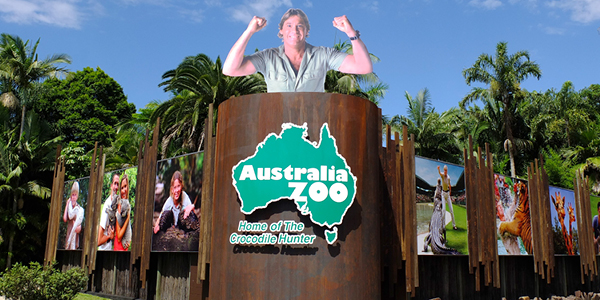
\includegraphics[width=\linewidth]{figures/au_zoo_example.jpg}
  \caption{Representative image $I$ for the anchor $v_0=\texttt{Australia\_Zoo}$.}
  \label{apdxfig:au-zoo-anchor}
  \vspace{-0.6em} 
\end{wrapfigure}

All three invariants of Eq.~\ref{eq:fuzz-invariants} are satisfied: $a$ is preserved, the descriptor combined with ``wife of'' resolves uniquely to Terri Irwin, and $q_f$ contains no surface form or alias of any node along $P$ (e.g.\ neither \texttt{Steve Irwin}, \texttt{Terri Irwin}, nor \texttt{The Crocodile Hunter} appears in $q_f$).

We then retrieve $K=8$ candidate images from Wikimedia Commons under the query \texttt{Australia\_Zoo} and rank them by CLIP~\citep{radford2021learning} cosine similarity to the canonical description \emph{``Australia Zoo entrance''}. The top-ranked image (Fig.~\ref{apdxfig:au-zoo-anchor}, similarity $0.34$) is selected as $I$. Replacing the anchor mention in $q_f$ with a visual referring expression yields the final VQA instance
\begin{equation*}
\begin{aligned}
(I,\ q,\ a) \;=\;& \bigl(\,I,\ \text{``On what date did the wife of the man who took over management of \emph{the zoo in}}\\
                 & \text{\emph{the image} in 1991 become an Australian citizen?''},\ \text{``20 November 2009''}\,\bigr).
\end{aligned}
\end{equation*}


The instance passes all four checks of Sec.~\ref{sec:vqa-construction}: \emph{masking} ($q$ contains no entity name or alias from $\{\texttt{Australia Zoo}, \texttt{Steve Irwin}, \texttt{Terri Irwin}\}$); \emph{uniqueness} (a GPT-4o judge given only $q$ returns exactly one consistent answer); \emph{visual relevance} (CLIP similarity $0.34$ exceeds our $0.28$ threshold); and \emph{non-triviality}, verified jointly under the filtering process of Sec.~\ref{sec:filtering-enhancement}.



\subsection{Counterfactual Design Choices}
\label{apdx:vqa-counterfactuals}

We probe the necessity of the three key design choices in Sec.~\ref{sec:vqa-construction} by counterfactually relaxing each one on the running example above.

\paragraph{Anchor $=$ Answer.}
Replacing $I$ with a photograph of Terri Irwin and asking for her citizenship date reduces the task to a single reverse-image lookup: \textsc{ImageSearch} on the new $I$ returns the Wikipedia page of Terri Irwin directly, from which the citizenship date is read off in one step. The multi-hop structure collapses, independently of how the question is phrased.

\paragraph{No fuzzing.}
Retaining the canonical $q_t$ as the final question---i.e.\ skipping the fuzzy-rewriting stage---exposes all entity names in plain text, and a single \textsc{TextSearch}(``Terri Irwin Australian citizenship date'') suffices to recover $a$. The image $I$ becomes decorative rather than load-bearing.

\paragraph{No hub avoidance.}
If the walk were allowed to admit the hub \texttt{Queensland} as a bridge, a natural descriptor such as ``the zoo located in [$v_j$]'' would fail the uniqueness check---thousands of zoos satisfy this relation---forcing either unsuccessful resampling or a contrived descriptor that itself leaks the identity of \texttt{Australia\_Zoo}. Hub avoidance (Appendix~\ref{apdx:wiki-sampling}) removes this failure mode at sampling time rather than relying on the downstream filters to catch it.


\section{System Prompts}
\label{apdx:system-prompts}

This section provides the complete system prompts used in \textsc{OpenSearch-VL}. The agent system prompt (Figure~\ref{apdxfig:agent-prompt}) is shared across inference and SFT data collection, and is paired with the machine-readable tool schema (Figure~\ref{apdxfig:tool-defs}) that is injected into the model context as \texttt{<tools>...</tools>} for OpenAI-style function calling. The two reward judge prompts (Figures~\ref{apdxfig:acc-judge} and~\ref{apdxfig:query-judge}) are used during RL training to compute $r_{\text{acc}}$ and $r_{\text{query}}$, respectively. For final benchmark reporting, we additionally adopt a GPT-4o judge prompt (Figure~\ref{apdxfig:bench-judge}) that is aligned with the evaluation protocol of Vision-DeepResearch~\citep{huang2026vision}, so that our numbers remain directly comparable to prior multimodal deep-research work.

\setcounter{figure}{7}
\begin{figure}[H]
\centering
\begin{promptbox}[prompttea]{Accuracy Reward Judge Prompt ($r_{\mathrm{acc}}$)}
You are an impartial judge evaluating whether a deep research report contains the correct answer.

[Question]
\{question\}

[Correct Answer]
\{reference\_answer\}

[Deep Research Report]
\{assistant\_answer\}

Task: Determine if the deep research report contains the correct answer anywhere in its content.

Instructions:
\begin{enumerate}[leftmargin=*,nosep]
\item Read through the entire research report carefully
\item Look for the correct answer anywhere in the report (it may be embedded in paragraphs, tables, or sections)
\item Check if the information in the report is consistent with the correct answer
\item The answer does NOT need to be in a specific format or labelled as ``final answer''
\item Provide your reasoning
\item Answer with ``yes'' if the report contains the correct answer, ``no'' if it doesn't or contradicts it
\end{enumerate}

Output format:
correct: [yes/no]
reasoning: [your explanation]
\end{promptbox}
\caption{The GPT-4o judge prompt used to compute the accuracy reward $r_{\text{acc}} \in \{0,1\}$ during RL training.}
\label{apdxfig:acc-judge}
\end{figure}

\setcounter{figure}{9}
\begin{figure}[htbp]
\centering
\begin{promptbox}[promptamber]{Benchmark Evaluation Judge Prompt (GPT-4o)}
You are an impartial judge evaluating whether a deep research report contains the correct answer.

[Question]
\{question\}

[Correct Answer]
\{correct\_answer\}

[Deep Research Report]
\{response\}

Task: Determine if the deep research report contains the correct answer anywhere in its content.

Instructions:
\begin{enumerate}[leftmargin=*,nosep]
\item Read through the entire research report carefully
\item Look for the correct answer anywhere in the report (it may be embedded in paragraphs, tables, or sections)
\item Check if the information in the report is consistent with the correct answer
\item The answer does NOT need to be in a specific format or labelled as ``final answer''
\item Provide your reasoning
\item Answer with ``yes'' if the report contains the correct answer, ``no'' if it doesn't or contradicts it
\end{enumerate}

Output format:
correct: [yes/no]
reasoning: [your explanation]
\end{promptbox}
\caption{GPT-4o judge prompt used for \emph{benchmark} evaluation of \textsc{OpenSearch-VL} and all baselines. We deliberately keep this prompt aligned with the evaluation protocol released by Vision-DeepResearch~\citep{huang2026vision}, so that reported accuracies are directly comparable across systems. Although structurally similar to the RL accuracy-reward judge (Figure~\ref{apdxfig:acc-judge}), this prompt is applied \emph{post-hoc} to final agent trajectories rather than as a training signal, and uses the field names (\texttt{question}, \texttt{correct\_answer}, \texttt{response}) consumed by our evaluation script.}
\label{apdxfig:bench-judge}
\end{figure}

\begin{figure}[H]
\centering
\begin{promptbox}[promptplum]{Query-Quality Reward Judge Prompt ($r_{\mathrm{query}}$)}
You are an impartial judge evaluating the quality and utility of an agent's search trajectory.

[Original Question]
\{question\}

[Ground Truth Answer]
\{ground\_truth\}

[Agent's Final Answer]
\{prediction\}

[Search Trajectory]
\{trajectory\_summary\}

[Evaluation Criteria]
Evaluate the overall utility of the agent's search queries and retrieved results:

\begin{enumerate}[leftmargin=*,nosep]
\item \textbf{Image search utility}: Did image searches retrieve visual evidence that genuinely supports answering the question? Were the images relevant, or just noise?
\item \textbf{Text search utility}: Did text searches find relevant textual information? Were queries well-formed and targeted?
\item \textbf{Query progression}: Did the queries show logical progression---refining, narrowing, or covering different aspects? Or did they repeat / drift aimlessly?
\item \textbf{Complementarity}: Did image and text searches complement each other, providing evidence that one modality alone couldn't supply?
\item \textbf{Evidence vs.\ noise ratio}: What fraction of retrieved results actually contained useful evidence versus irrelevant content?
\end{enumerate}

Score the overall query utility from 0.0 to 1.0:
- 0.0: No useful information retrieved; all searches irrelevant or failed
- 0.3: Mostly noise with occasional marginally relevant results
- 0.5: Mixed---some useful evidence found but significant noise or inefficiency
- 0.7: Good search strategy; majority of results were relevant
- 1.0: Excellent---targeted, efficient queries that retrieved highly relevant evidence

Output format (strictly follow):
score: [a single float between 0.0 and 1.0]
reasoning: [brief explanation in 2--3 sentences]
\end{promptbox}
\caption{The GPT-4o judge prompt used to compute the query-quality reward $r_{\text{query}} \in [0,1]$ during RL training.}
\label{apdxfig:query-judge}
\end{figure}

\setcounter{figure}{6}
\begin{figure}[htbp]
\centering
\begin{promptbox}[promptblue]{Agent System Prompt (Inference / SFT Data Collection)}
You are an advanced \textbf{Visual Investigation Agent}. Answer user questions with maximum precision by proactively using image-processing and retrieval tools.

\textbf{Core Philosophy: ``Verify, Don't Guess''}
\begin{enumerate}[leftmargin=*,nosep]
\item \textbf{Tool-First Mindset}: small text $\Rightarrow$ \texttt{crop}; blurry $\Rightarrow$ \texttt{sharpen}; tilted $\Rightarrow$ \texttt{perspective\_correct}. Never rely on the internal encoder when a tool gives a sharper view.
\item \textbf{Chain Your Tools}: non-trivial queries usually require a pipeline, e.g.\ \texttt{perspective\_correct}~$\rightarrow$~\texttt{crop}~$\rightarrow$~\texttt{layout\_parsing}.
\item \textbf{External Validation}: whenever the answer depends on facts not purely visible in the pixels, you \emph{must} call \texttt{text\_search}.
\end{enumerate}

\textbf{1. Tool Calling Format}

Function signatures are provided inside \texttt{<tools>...</tools>}. Emit tool calls as one JSON object inside\\
\texttt{<tool\_call>\{"name": <f>, "arguments": <args>\}</tool\_call>}, one call per turn.

\textbf{2. Your Toolbox}

\textcolor{red}{\textbf{\{Tool List\}}}

For each of the seven tools the production prompt specifies its \emph{trigger} (when to call), \emph{params} (JSON schema), and \emph{output} (how to consume the return value). The tools fall into three families: \emph{visual perception} (\texttt{crop}, \texttt{layout\_parsing}); \emph{image enhancement} (\texttt{perspective\_correct}, \texttt{super\_resolution}, \texttt{sharpen}); and \emph{knowledge retrieval} (\texttt{text\_search}, \texttt{image\_search}; image search must be followed by text search).

\textbf{3. Thinking Protocol}

Before any action, emit a \texttt{<think>} block with: (i) \emph{analyse request}; (ii) \emph{assess image quality}---legibility, geometry, and target size, mapping any deficiency to the corresponding enhancement tool; (iii) \emph{identify information gaps}---retrieval needed?; (iv) \emph{formulate plan}---commit to a single next action.

\textbf{Critical reminders}: (a) when \texttt{layout\_parsing} returns text, treat it as ground truth---do \emph{not} fall back to visual guessing; (b) after \texttt{image\_search}, always call \texttt{text\_search} for factual detail; (c) \texttt{text\_search} summaries are already query-focused---trust them and cite the returned URLs.

\textbf{4. Workflow Recipes}
\begin{itemize}[leftmargin=*,nosep]
\item \emph{Unreadable document}: \texttt{perspective\_correct}~$\rightarrow$~\texttt{sharpen}~$\rightarrow$~\texttt{layout\_parsing}.
\item \emph{Dense chart}: \texttt{crop} (region of interest)~$\rightarrow$~\texttt{layout\_parsing}.
\item \emph{Entity identification}: \texttt{image\_search}~$\rightarrow$~\texttt{text\_search} (mandatory follow-up).
\end{itemize}

\textbf{5. Output Rules}
\begin{enumerate}[leftmargin=*,nosep]
\item \textbf{Single action per turn}; wait for its result before the next.
\item \textbf{Think first}: never emit \texttt{<tool\_call>} without a preceding \texttt{<think>}.
\item \textbf{Image refs}: initial image is \texttt{img\_1}; each tool output yields \texttt{img\_2}, \texttt{img\_3}, \ldots; always operate on the latest best version.
\item \textbf{Final answer}: emit \texttt{<response>...</response>} once evidence suffices.
\end{enumerate}

\textbf{6. Execution Example} (tool-use turn)
\begin{flushleft}\ttfamily\footnotesize
<think> Invoice img\_1 is skewed; correct perspective first. </think>\\
<tool\_call>\{"name": "perspective\_correct", "arguments": \{"image": "img\_1"\}\}</tool\_call>
\end{flushleft}
\end{promptbox}
\caption{Condensed agent system prompt used during both inference and SFT trajectory collection. The placeholder \textcolor{red}{\textbf{\{Tool List\}}} stands in for the per-tool description block of the production prompt; concrete \emph{trigger}/\emph{params}/\emph{output} content for each of the seven tools is reproduced in Figure~\ref{apdxfig:tool-defs} (machine-readable schema) and Table~\ref{tab:search-tools} (human-readable summary). Relative to the original prompt used in our codebase, we condense the three long ``critical reminder'' paragraphs into a single line, drop redundant execution examples, and merge per-tool workflow sub-rules into the core philosophy; no behavioural rule is removed.}
\label{apdxfig:agent-prompt}
\end{figure}



\begin{figure}[htbp]
\centering
\begin{toolsjson}{Tool Definitions (OpenAI-compatible JSON schema, injected as \texttt{<tools>})}
{
  "tools": [
    {
      "type": "function",
      "function": {
        "name": "crop",
        "description": "Crop a region from an image; trigger when target covers < 30% of the frame.",
        "parameters": {
          "type": "object",
          "properties": {
            "image":  {"type": "string",  "description": "Image reference, e.g. 'img_1'"},
            "x":      {"type": "integer", "description": "Top-left X coordinate"},
            "y":      {"type": "integer", "description": "Top-left Y coordinate"},
            "width":  {"type": "integer", "description": "Width of the crop region"},
            "height": {"type": "integer", "description": "Height of the crop region"}
          },
          "required": ["image", "x", "y", "width", "height"]
        }
      }
    },
    {
      "type": "function",
      "function": {
        "name": "text_search",
        "description": "Serper + JINA Reader + Qwen3-32B summarisation over top-k web pages.",
        "parameters": {
          "type": "object",
          "properties": {
            "q":     {"type": "string",  "description": "Search query keywords"},
            "hl":    {"type": "string",  "description": "Language code", "default": "en"},
            "top_k": {"type": "integer", "description": "#results to summarise", "default": 5}
          },
          "required": []
        }
      }
    },
    // ---- Remaining tools follow the same schema; full specs in the tool-suite table ----
    { "function": { "name": "layout_parsing",      "required": []         } },
    { "function": { "name": "perspective_correct", "required": ["image"]  } },
    { "function": { "name": "super_resolution",    "required": ["image"]  } },
    { "function": { "name": "sharpen",             "required": ["image"]  } },
    { "function": { "name": "image_search",        "required": ["url"]    } }
  ]
}
\end{toolsjson}
\caption{Machine-readable tool schema produced by our agent codebase and injected into the model context as an OpenAI-style \texttt{<tools>} block. Two representative tools (\texttt{crop} for visual perception and \texttt{text\_search} for knowledge retrieval) are shown in full; the remaining five follow the same schema and are collapsed to their \texttt{name}/\texttt{required} fields---their complete specifications are listed in Table~\ref{tab:search-tools}. At inference time the agent emits tool calls inside \texttt{<tool\_call>\{"name": \ldots, "arguments": \ldots\}</tool\_call>} conforming to the \texttt{parameters} schema.}
\label{apdxfig:tool-defs}
\end{figure}

\FloatBarrier

\section{Tool Definition and Usage}
\label{apdx:tool-definition}

This section details the search-oriented tools integrated within \textsc{OpenSearch-VL}. For each tool, we articulate its core functionality, formalize its input--output signature, describe its backend implementation, and contextualize its operational role within visual search trajectories. The tool set is partitioned into three functional modalities: \emph{Retrieval}, \emph{Image Enhancement}, and \emph{Attention \& Parsing}. Retrieval tools interface with the open web via remote APIs; image enhancement tools operate as lightweight, deterministic local primitives; and attention \& parsing tools combine local spatial priors with remote document-understanding services.

\subsection*{Retrieval Tools}

\begin{itemize}[leftmargin=*,itemsep=5pt]

    \item \textbf{\textsc{TextSearch}}
    \begin{itemize}
        \item \textbf{Functionality:} A composite textual retrieval mechanism comprising three pipelined stages: (i) a Serper-backend search query to retrieve top-$k$ candidate URLs; (ii) a JINA Reader invocation to fetch and normalize the HTML payloads into clean Markdown; and (iii) a Qwen3-32B summarization pass that distills a query-focused 2--4 sentence synopsis per document. The terminal output is a structured list of \texttt{[Passage $i$] (title, url, summary)} objects.
        \item \textbf{Operational Role:} Functions as the primary ``read the web'' primitive when surface-level snippets are insufficient. It is indispensable for resolving complex, multi-hop knowledge queries and retrieving long-tail factual evidence that necessitates reasoning over entire paragraphs.
    \end{itemize}

    \item \textbf{\textsc{ImageSearch}}
    \begin{itemize}
        \item \textbf{Functionality:} A visual-entity and reverse-image search tool powered by the Polaris Lens API. It accepts a publicly routable image URL and returns a structured JSON payload encompassing visually similar images, recognized entities, related domain URLs, and textual captions associated with the query image.
        \item \textbf{Operational Role:} Serves as the critical bridge transmuting purely visual queries into retrievable textual entities. When the agent determines that resolving a query hinges on identifying an unknown visual entity (e.g., a landmark, logo, or public figure), it invokes \textsc{ImageSearch} to extract external semantic grounding, which can subsequently be cross-referenced via \textsc{TextSearch}.
    \end{itemize}

\end{itemize}

\subsection*{Image Enhancement Tools}

\begin{itemize}[leftmargin=*,itemsep=5pt]

    \item \textbf{\textsc{Sharpen}}
    \begin{itemize}
        \item \textbf{Functionality:} A deterministic deblurring operator implemented via OpenCV Unsharp Masking. Parameterized by an input image and an optional sharpening intensity $\alpha$ (default $1.5$), it computes the enhanced image $I_{\text{out}} = (1{+}\alpha)\,I - \alpha\,G_\sigma * I$, where $G_\sigma$ is a Gaussian blur kernel.
        \item \textbf{Operational Role:} Deployed when the input image exhibits pervasive blur or soft edge gradients, which frequently degrade downstream optical character recognition (OCR) or object detection. As a computationally cheap, side-effect-free preprocessing step, the agent can heuristically apply \textsc{Sharpen} prior to reinvoking perceptual tools.
    \end{itemize}

    \item \textbf{\textsc{SuperResolution}}
    \begin{itemize}
        \item \textbf{Functionality:} A deep-learning-based upscaling tool employing the EDSR architecture via OpenCV's \texttt{dnn\_superres} module. It accepts an image and a discrete scale factor (default $\times 4$), emitting a high-resolution reconstruction. For robustness, if the EDSR weights are unavailable in the deployment environment, it gracefully degrades by returning the original image.
        \item \textbf{Operational Role:} Crucial for mitigating resolution bottlenecks, particularly on tightly cropped patches or inherently low-fidelity inputs (e.g., thumbnails). By synthesizing high-frequency details, it substantially elevates the reliability and extraction accuracy of subsequent \textsc{OCR} invocations.
    \end{itemize}

    \item \textbf{\textsc{PerspectiveCorrect}}
    \begin{itemize}
        \item \textbf{Functionality:} An automated perspective-rectification primitive. It executes a Canny edge detection pipeline on the grayscale projection, extracts the maximal quadrilateral contour, and computes a four-point perspective transform to warp the image into a fronto-parallel plane. If a reliable quadrilateral cannot be established, it falls back to the original image alongside a diagnostic warning.
        \item \textbf{Operational Role:} Addresses the pervasive domain shift of real-world captures, such as skewed photographs of documents, receipts, or screens. Rectifying the image geometry dramatically improves the bounding-box precision and text-recognition fidelity of downstream \textsc{OCR} parsing.
    \end{itemize}

\end{itemize}

\subsection*{Attention and Parsing Tools}

\begin{itemize}[leftmargin=*,itemsep=5pt]

    \item \textbf{\textsc{Crop}}
    \begin{itemize}
        \item \textbf{Functionality:} A deterministic spatial-attention primitive. Parameterized by an image and a bounding box coordinate tuple $(x, y, w, h)$, it extracts and isolates the specified rectangular sub-region, writing the artifact to disk for subsequent reference.
        \item \textbf{Operational Role:} Models the human cognitive mechanism of foveating onto a dense sub-region within a cluttered scene (e.g., isolating a single chart in a multi-panel figure). It is the canonical mechanism for the policy to suppress peripheral noise prior to passing a clean, localized patch to downstream tools such as \textsc{OCR}, \textsc{SuperResolution}, or \textsc{ImageSearch}.
    \end{itemize}

    \item \textbf{\textsc{OCR}}
    \begin{itemize}
        \item \textbf{Functionality:} A layout-aware optical character recognition service backed by a remote PaddleX infrastructure. It consumes a base64-encoded image alongside optional flags for chart-recognition and document-orientation classification. It emits a hierarchical list of detected text blocks (categorized into titles, body text, footnotes, etc.), yielding explicit \texttt{block\_label}, \texttt{block\_content}, and a reading-order-reconstructed \texttt{formatted\_text}.
        \item \textbf{Operational Role:} Serves as the agent's primary ``read the image'' capability. Beyond plain character recognition, its preservation of the document's logical layout is indispensable for queries dependent on structural hierarchy (e.g., distinguishing a figure caption from a section title). It is optimally invoked following upstream enhancements (\textsc{PerspectiveCorrect}, \textsc{Sharpen}, \textsc{SuperResolution}) or spatial isolation (\textsc{Crop}).
    \end{itemize}

\end{itemize}

\section{Case Study}

Figure~\ref{fig:case-study} presents a representative end-to-end trajectory of \textbf{OpenSearch-VL} on a knowledge-intensive visual question (``\emph{In what year did this bridge open?}''), whose answer is recoverable neither from the encoder's parametric knowledge nor from any single retrieval call. The agent first dispatches a \textsc{Crop} on the roadside signage to foveate on the most diagnostic sub-region, forwards the cropped patch to \textsc{ImageSearch} to identify the structure as the \textit{Kessock Bridge}, and then issues a targeted \textsc{TextSearch} that corroborates the opening year as \textbf{1982}. The trace exemplifies the compositional ``verify, don't guess'' behavior that the visual--retrieval action space $\mathcal{T}_v \cup \mathcal{T}_s$, the query-quality reward $r_{\text{query}}$, and the fatal-aware masking scheme are jointly designed to incentivize: tools are chained in an order that progressively grounds the question, and the rollout terminates as soon as cross-modal evidence converges.

\begin{figure}[htbp]
  \vspace{20pt}
  \centering
  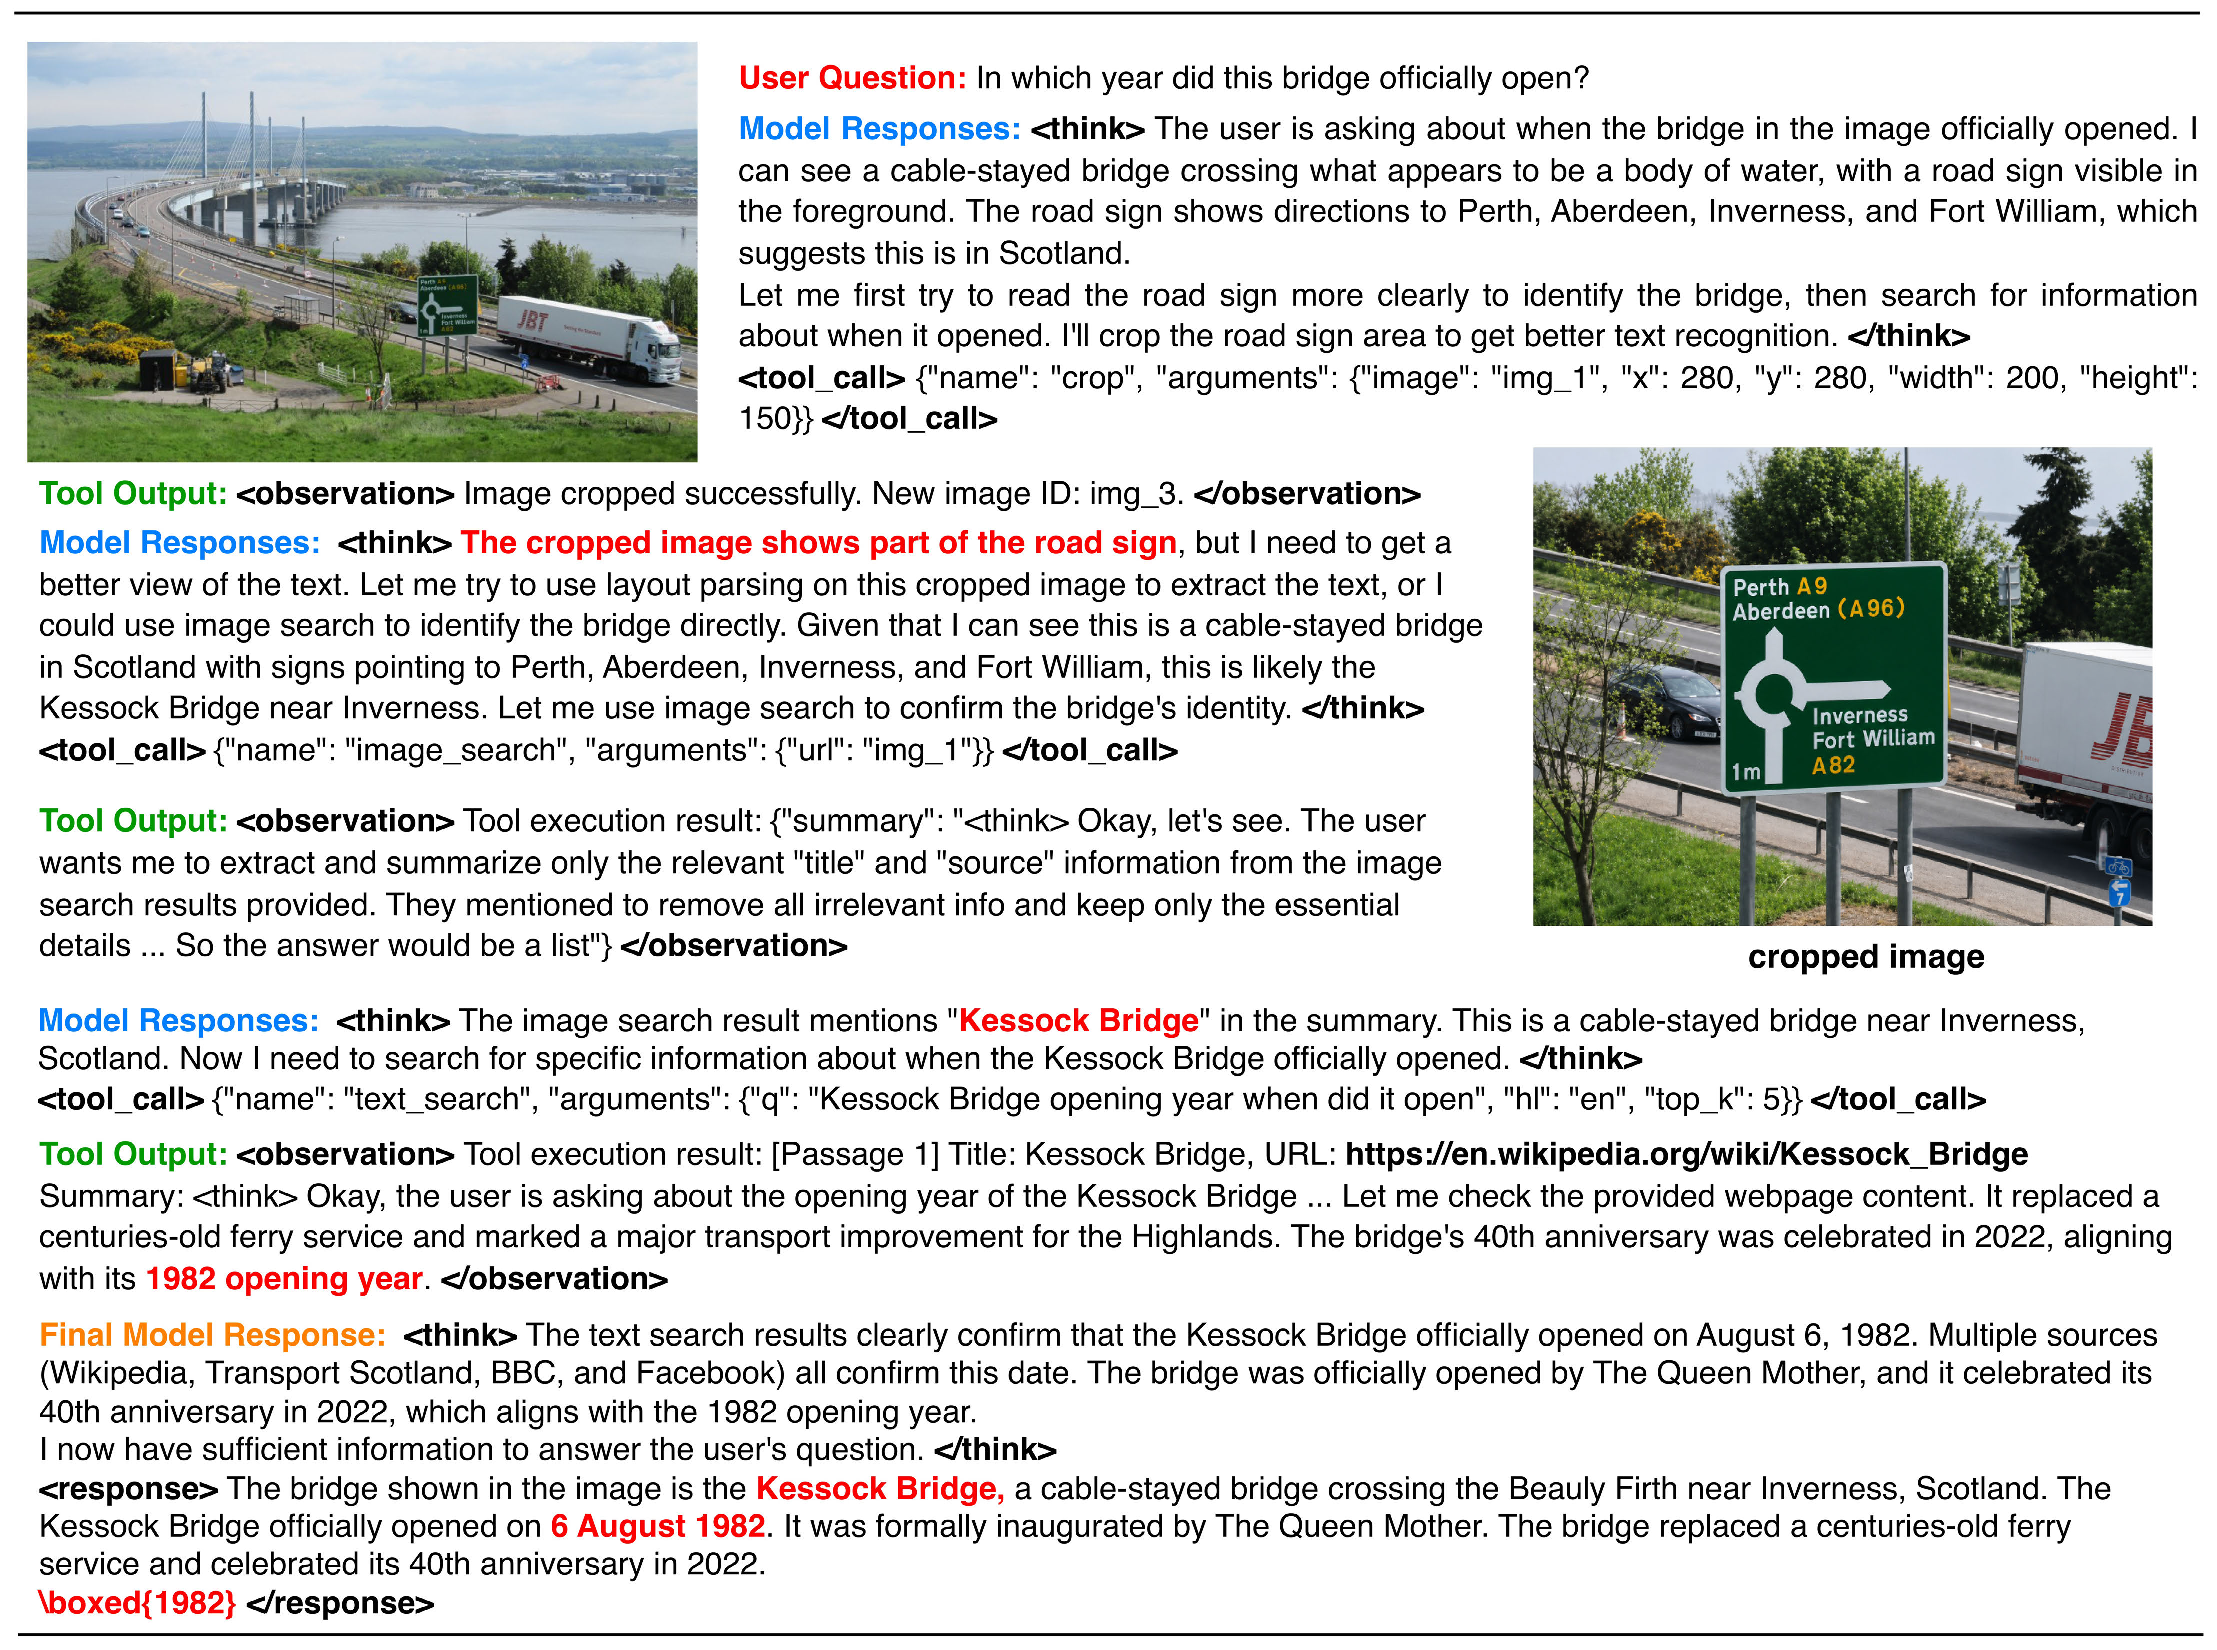
\includegraphics[width=\linewidth]{figures/case_v1.pdf}
  \caption{\textbf{Case study of \textbf{OpenSearch-VL}.}
  Given an image-based question about the opening year of a bridge, the model first inspects visual evidence and crops the road sign to obtain finer-grained location cues. It then uses image search to identify the bridge as the Kessock Bridge and issues a targeted text search to verify its official opening date. The retrieved evidence confirms that the bridge opened in 1982, leading to the final answer. This example illustrates how interleaved visual inspection, image retrieval, and textual evidence acquisition can resolve knowledge-intensive visual questions.}
  \label{fig:case-study}
\end{figure}



\stopcontents[appendix]% close the appendix-only TOC scope (paired with \startcontents above)


